\documentclass{article}
\usepackage[utf8]{inputenc}
\usepackage[left=17mm, top=17mm, right=17mm, bottom=15mm, nohead, nofoot]{geometry}
\usepackage{enumitem}
\usepackage{graphicx}
\twocolumn



\setlist[itemize]{itemsep=0pt, parsep=0pt, partopsep=0pt, topsep=1.4pt}
\setcounter{page}{272}

\begin{document}

The parameters are defined as shown below:
\begin{itemize}
    \item $ T_{sc}(u)$ --  all substructures after the decomposition of the user answers $u$;
    \item $ T_{sc}(s)$ -- all substructures after the decomposition of the standard answers $s$;
    \item $\otimes$ -- binary matching operator, which represents the number of matching substructures in the set of two substructures.
\end{itemize}

Once the similarity between the answers is obtained, the
correctness and completeness of the user answers can be
verified by combining it with the corresponding evaluation
strategy. The evaluation strategy of the objective questions
is shown below:
\begin{itemize}
   \item if there is only one correct option for the current test question, only if the standard answer and the user answer match exactly, the user answer is considered correct;
   \item if the current question has multiple correct options:
        \begin{itemize}
            \item as long as the user answer contains an incorrect option, the user answer is considered incorrect;
            \item  if all the options in the user answer are correct, but the number of correct options is less than the number of correct options in the standard answer, the user answer is considered correct but incomplete. At this time, the user answer score is $R_{sc}*Max_{score}$;
            \item if all the options in the standard answer match exactly with all the options in the user answer, the user answer is exactly correct.
        \end{itemize}
\end{itemize}

Fig. 1 shows an example of verification of user answer
to judgment question in SCg-code.

\small\begin{figure}[h]
    \centering
    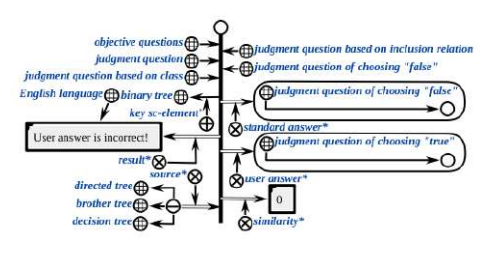
\includegraphics{picture.png}
    \caption  {An example of verification of user answer to judgment question.}
    \label{fig:mpr}
\end{figure}

\noindent\textit{D. Verification of answers to subjective questions}

The approach to calculating the similarity between the semantic graphs of answers to subjective questions, according to the knowledge description structure of the different types of subjective questions, has been divided into: 1. the approach to calculating the similarity between answers to definition explanation questions; 2. the approach to calculating the similarity between answers to proof questions and problem-solving task.


\textbf{Calculating the similarity between answers to
definition explanation questions}

The answers to the definition explanation questions are described based on logical formulas (SCL-code). Logic formulas are powerful tools for formal knowledge representation in the framework of OSTIS Technology, which are expanded based on the first-order predicate logic formulas [5]. In the process of calculating the similarity between the semantic graphs of answers to this type of test question, the following tasks need to be solved:
\begin{itemize}
    \item establishing the mapping relationship of potential equivalent variable sc-node pairs between the semantic graphs of the answers;
    \item calculating the similarity between semantic graphs;
    \item  if the similarity between semantic graphs is not equal to 1, they also need to be converted to the prenex normal form (PNF) representation separately, and then the similarity between them is calculated again [23].
\end{itemize}

The semantic graphs of answers to the definition
explanation questions are constructed based on logical
formulas, the variables sc-nodes (bound variables) are
included in the semantic graphs. In order to calculate the
similarity between semantic graphs, mapping relationship
of potential equivalent variable sc-node pairs between
them needs to be established

In the ostis-systems, the sc-construction composed of
sc-tuple, relation sc-node, role relation sc-node and scconnector is used to describe logical connectives (such
as negation ($\neg$) and implication ($\rightarrow$), etc.) and quantifiers (universal quantifier ($\forall$) and existential quantifier ($\exists$)), atomic logic formula (various sc-constructions) or multiple atomic logic formulas that satisfy conjunctive relation are contained in the sc-structure and connected with the corresponding sc-tuple, and these sc-elements together constitute the semantic graph of answers to the definition explanation questions. Its structure is a tree.

If the standard answer and the user answer are exactly equal, it means that the atomic logic formulas with the same semantics between the answers have the same position in the semantic graph. Thus a mapping relationship between variables sc-nodes can be established by determining the position in the semantic graph of each sc-construction containing the variable sc-nodes and the semantic connotation it expresses [20], [21], [22].

The process of establishing the mapping relationship of the potential equivalent variable sc-node pairs between answers is shown below:
\begin{itemize}
    \item each sc-tuple and sc-structure in the semantic graph is numbered separately according to the depth-first search strategy (DFS), (for indirectly determining the position of variables sc-nodes in the semantic graph);
\end{itemize}

\end{document}
